\subsection{Modularisierung}
    Der Programmcode wurde modulweise erstellt, sodass Themengebiete 
    voneinander abgekapselt sind. Durch geschicktes Einbinden kann somit
    Codeverdoppelung vermieden werden.

    \subsubsection{Modulübersicht}

        \paragraph{twi.h}
            Das \textit{Two Wire Interface (TWI)} Modul stellt
            Funktionen zu Verfügung um über ein \textit{TWI}-Bus-System zu 
            kommunizieren. Dabei wurde das Modul sehr \textit{Low-Level}
            gehalten. Das bedeutet unter anderem, dass der Klient dieses Modules 
            selber dafür verantwortlich ist \textit{Start} und \textit{Stop} 
            Konditionen auf den Bus zu setzen. Dabei ist zu beachten, dass dieses
            Modul blockierend arbeitet.

            \begin{figure}[H]
                \centering
                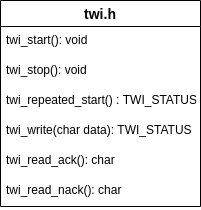
\includegraphics[scale=0.6]{img/twi.png}
                \caption{twi.h}
            \end{figure}

        \paragraph{led.h}
            Das LED Modul stellt Funktionen rund um die LED Steuerung zu Verfügung.
            Hiermit lässt sich die die LED ein- und ausschalten sowie die Farbe
            konfigurieren und das Blinkverhalten einstellen.

            \begin{figure}[H]
                \centering
                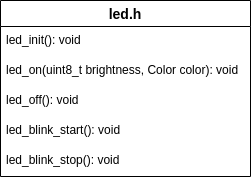
\includegraphics[scale=0.6]{img/led.png}
                \caption{led.h}
            \end{figure}

        \paragraph{timer.h}
            In dem Timer Modul finden sich Funktionen um den Timer zu steuern, der
            die Abschaltverzögerung implementiert.

            \begin{figure}[H]
                \centering
                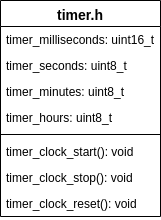
\includegraphics[scale=0.6]{img/timer.png}
                \caption{timer.h}
            \end{figure}

        \paragraph{mpu6050.h}
            Dieses Modul bietet \textit{High-Level} Funktionen um die Daten
            des Accelerometers zu erhalten sowie Konfigurationsmöglichkeiten.
            
            \begin{figure}[H]
                \centering
                
\includegraphics[scale=0.6]{img/mpu.png}
                \caption{mpu6050.h}
            \end{figure}

        \paragraph{config.h}
            Das config Modul bietet Konstanten zur Konfiguration der Kerze.
            So können alle Voreinstellungen bearbeitet werden und an die
            entsprechenden Anforderungen angepasst werden.

        \paragraph{types.h}
            Das types Modul beinhaltet alle Datenstrukturen die für das Programm 
            benötigt werden (Siehe \ref{Datenstrukturen}).

        \paragraph{debug.h}
            Das Debug Modul wird zu debug Zwecken benötigt und implementiert
            somit nur Funktionen um über die \textit{USART} Schnittstelle Daten zu
            senden, jedoch nicht um Daten zu empfangen. Die Daten können dann von einer
            seriellen Schnittstelle an einem Computer betrachtet werden.
            Das Modul arbeitet hierbei blockierend.

            \begin{figure}[H]
                \centering
                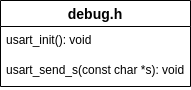
\includegraphics[scale=0.6]{img/debug.png}
                \caption{debug.h}
            \end{figure}
    
    \subsubsection{Programmorganisationsplan}
        \begin{figure}[H]
            \centering
            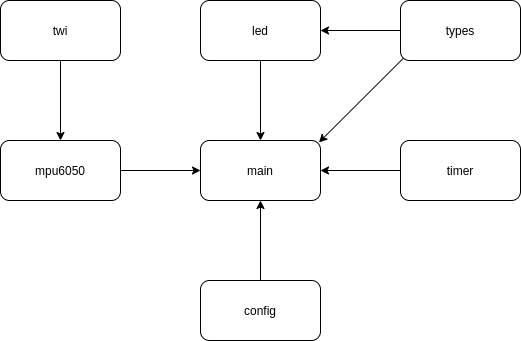
\includegraphics[scale=0.5]{img/pop.png}
            \caption{Programmorganisationsplan}
        \end{figure}

